\chapter{Measurements}
\label{chapter:measurements}
\section{Introduction to Measurements}
Measuring a design gives real-world insight into the success of a design of a component. Circuit theory does not always match what happens in the real world, as assumptions are made to simplify models on paper. Therefore, testing and measuring real-world data is essential to the design of a system, as it can point out flaws in the assumptions made by the theory. This, therefore, allows for adjustments to be made, which would only be found by measuring.

\section{Measurements Results}
\subsection{Power Supply}
The voltage waveform across load resistors $R_{\text{load},1}$ and $R_{\text{load},2}$ were measured under four distinct conditions to evaluate the ripple voltage. During these measurements, only the positive side of the power supply was loaded, as the negative side is an exact replica of the positive side due to the symmetry of a center-tapped transformer (CT-T). The measurements were performed by connecting the probe to both the ground and the positive output of the power supply, denoted by $V_{out}$, with the voltage being measured across the load resistors. These measurements yielded the characteristics shown in Tab. \ref{tab:CharacteristicsSim}. The ripple was calculated using Eq. \ref{RippleVoltageEquation}. The code provided in Appendix \ref{sec:ripvoltcodemea} was utilized to calculate the values presented in Tab. \ref{tab:CharacteristicsSim}.

\begin{figure}[H]
    \centering
    \captionsetup{justification=raggedright, labelfont=bf}
    \resizebox{0.75\columnwidth}{!}{%
        \begin{tikzpicture} 
        \pgfplotsset{
                every axis legend/.append style={at={(0.98,0.02)}, anchor=south east, legend columns=1},
                every axis/.append style={
                    grid=major,
                    grid style={line width=0.5pt, draw opacity=0.4},
                    tick align=inside, % Ticks will now be inside the plot
                    minor tick num=5
                }
            }
            \begin{axis} [
                xlabel={Time [s]}, % Adjusted x-axis label
                ylabel={$V_{\text{out}}$ [V]},
                title={Effect of different load resistances on $V_{\text{out}}$},
                width=\textwidth,
                height=0.6\textwidth,
                xticklabel style={/pgf/number format/.cd, fixed, fixed zerofill, precision=3}, % Force fixed-point notation
                scaled x ticks=false, % Disable automatic scaling
                xtick scale label code/.code={}, % Ensure no scale label is shown
                enlargelimits=true % Ensure the graph has enough space for ticks
            ]
                % Plot for 19Ω
                \addplot+[black, no markers] 
                    table [x=d, y=e, col sep=comma] {TU Delft Booming Bass Project Report/appendix/csv/19 ohm/F0009CH1.CSV};
                \addlegendentry{$V_{\text{out}}$ with 19$\Omega$}

                % Plot for 38Ω
                \addplot+[blue, no markers] 
                    table [x=d, y=e, col sep=comma] {TU Delft Booming Bass Project Report/appendix/csv/38 ohm/F0007CH1.CSV};
                \addlegendentry{$V_{\text{out}}$ with 38$\Omega$}

                % Plot for 76Ω
                \addplot+[red, no markers] 
                    table [x=d, y=e, col sep=comma] {TU Delft Booming Bass Project Report/appendix/csv/76 ohm/F0011CH1.CSV};
                \addlegendentry{$V_{\text{out}}$ with 76$\Omega$}

                % Plot for no load
                \addplot+[green, no markers] 
                    table [x=d, y=e, col sep=comma] {TU Delft Booming Bass Project Report/appendix/csv/No load/F0008CH1.CSV};
                \addlegendentry{$V_{\text{out}}$ with no load}
            \end{axis}
        \end{tikzpicture}%
    }
    \caption{The output voltage $V_{out}$ waveform for various load resistances: 19$\Omega$, 38$\Omega$, 76$\Omega$ and no load. As the load resistance $R_{load}$ increases, the ripple $u_{\text{ripple}}$ decreases. This occurs because a high load resistance reduces the current drawn from the power supply, causing the voltage across the smoothing capacitor to remain more stable and preventing large fluctuations in the output voltage. This results in a smaller ripple as the capacitor has more time to charge and discharge gradually.}
    \label{fig:MeasuredLoadOutputVoltage}
\end{figure}


\begin{figure}[H]
    \centering
    \begin{minipage}{0.48\textwidth}
        \centering
        \begin{threeparttable}
          \centering
          \begin{tabular}{c @{\hspace{12pt}} *4{c} S @{\hspace{12pt}}}
            \toprule
            \multicolumn{5}{c}{\textbf{Measured Power Supply Characteristics}} \\
            \cmidrule(lr){1-5}
            & & \multicolumn{3}{c}{\textbf{Performance Metrics}} \\
            \cmidrule(lr){3-5}
            & $R_\text{Load}$ [$\Omega$] & $V_\text{Av.}$ [V] & $I_\text{res}$ [A] & $u_\text{ripple}$ [\%] \\
            \midrule
            1 & 19 & 20.1 & 1.06 & 3.23 \\
            2 & 38 & 21.1 & 0.56 & 1.66 \\
            3 & 76 & 21.9 & 0.29 & 1.10 \\
            4 & Open & 23.0 & 0.00 & 0.26 \\
            \bottomrule
          \end{tabular}
        \end{threeparttable}
        \captionsetup{justification=raggedright, labelfont=bf}
        \caption{Characteristics of the power supply in real-world applications under various load levels, using load resistors equipped with large heatsinks to dissipate the thermal energy from imperfect energy conversion. The data includes each load's average output voltage, current, and ripple percentage.}
        \label{tab:CharacteristicsSim}
    \end{minipage}\hfill
    \begin{minipage}{0.48\textwidth}
        \centering
        \resizebox{\linewidth}{!}{%
            \begin{tikzpicture} 
                \pgfplotsset{
                    every axis legend/.append style={ at={(0.02,0.98)}, anchor=north west, legend columns = 1}, 
                    every axis/.append style={ytick distance=0.25, xtick distance=2, minor tick num=1, grid=major,
                    every axis grid/.append style={line width=0.5pt, draw opacity=0.4}}}
                    \begin{axis} [xlabel = {Delivered power [W]}, ylabel = {Ripple [\%]}]
                        \addlegendentry{Ripple[\%]}
                        \addplot+[no markers] table[row sep=crcr] {
                            Supplied power(W):       Ripple(\%): \\  
                            21.31       3.23  \\
                            11.82     1.66  \\
                            6.351     1.10  \\
                            0     0.26  \\
                        };
                    \end{axis}
            \end{tikzpicture}%
        }
        \captionsetup{justification=raggedright, labelfont=bf}
        \caption{The output voltage ripple as a function of the power delivered to varying load resistances, showing the voltage ripple magnitude and the corresponding load power.}
        \label{fig:OutputVoltageRipplePower}
    \end{minipage}
\end{figure}
The ripple observed for the open circuit is likely due to a measurement error from the oscilloscope, which was set with a resolution of 0.04V. In the measurements, the maximum voltage recorded was 23.04V, while the average voltage was 23.00V. Although a small ripple could have resulted from the capacitors slowly discharging through the discharge resistors, the ripple induced by this current was negligible and thus insignificant compared to the one measured, as the discharge current is very small.
\subsubsection{Discharge Capacitors}

\begin{figure}[H]
    \centering
    \captionsetup{justification=raggedright, labelfont=bf}
    \resizebox{0.9\columnwidth}{!}{%
        \begin{tikzpicture} 
        \pgfplotsset{
                every axis legend/.append style={at={(0.98,0.02)}, anchor=south east, legend columns=1},
                every axis/.append style={
                    grid=major,
                    grid style={line width=0.5pt, draw opacity=0.4},
                    tick align=inside, % Ticks will now be inside the plot
                    minor tick num=5
                }
            }
            \begin{axis} [
                xlabel={Time [s]}, % Adjusted x-axis label
                ylabel={$V_{\text{out}}$ [V]},
                title={Effect of the smoothing capacitors on $V_{\text{out}}$},
                width=\textwidth,
                height=0.6\textwidth,
                xticklabel style={/pgf/number format/.cd, fixed, precision=0}, % Remove decimals by setting precision to 0
                enlargelimits=true % Ensure the graph has enough space for ticks
            ]
                \addplot+[no markers] table [x=d, y=e, col sep=comma] {TU Delft Booming Bass Project Report/appendix/csv/discharge/F0010CH1.CSV};
                \addlegendentry{\(V_{out}\)}
                \addplot[color=red] table[row sep = crcr]{0 8.829 \\ 249.8 8.829 \\};
                \addlegendentry{\(V_{e^{-1}}\)}
            \end{axis}
        \end{tikzpicture}%
    }
    \caption{The discharge curve of the capacitors, measured at $V_{\text{out}}$. The input voltage $V_{in}$ is disconnected from the power supply circuit at $t=33.0\text{s}$}
    \label{fig:dischargeCurve}
\end{figure}

From \autoref{fig:dischargeCurve}, it is evident that the capacitors are disconnected from the power supply at approximately $t=33.0\text{s}$. The discharge curve intersects the red line - indicating the point where $\tau=1$ - at around $\tau\approx 62\text{s}$. This implies that the time constant $\tau$ is approximately 28 seconds. Based on this, the capacitors are expected to fully discharge after 145 seconds, aligning well with the 2.5-minute discharge limit specified in the design requirements.

\subsection{Power Amplifier}
\label{section: measurements poweramp}
After simulating the circuit in LTSpice, it is crucial to test the power amplifier in a real-world environment to assess its actual performance. To achieve this, measurements must be conducted on the constructed power amplifier circuit. The expected outcome from this measurement is a Bode plot that accurately represents a band-pass filter with a dB gain of 27.82 dB and corner frequencies at 20.1Hz and 40.3kHz, corresponding to the -3dB of the gain. Additionally, it is anticipated that the DC offset of the operational amplifier will be amplified by no more than a factor of 1 in accordance with the design specifications. These measurements will provide valuable insights into the circuit's practical performance, ensuring that the theoretical predictions align with real-world behavior.

During the construction of the circuit, each resistor and capacitor was tested to ensure that the physical components matched the expected values from the simulations and calculations. This step was necessary because the capacitance of a capacitor can vary by approximately 20\% from the labeled value and the value of a resistor can vary anywhere from 0.1\% to 20\%. The measured values for all components can be seen in \stautoref{tab:Real values}. These are the same values as shown in \stautoref{tab: B2-1 actual ideal values} and \stautoref{tab:B2-1 ideal values}.
\begin{table}[H]
    \centering
    \begin{tabular*}{0.35\textwidth}{@{\extracolsep{\fill}} c c @{}}
        \toprule
        \textbf{Component} & \textbf{Value of Component} \\
        \midrule
        \textbf{$C_1$} & 166.5nF \\
        \textbf{$C_a$} & 40.5nF \\ 
        \textbf{$C_x$} & 986nF \\
        \textbf{$R_a$} & 987$\Omega$ \\
        \textbf{$R_b$} & 81.8k$\Omega$ \\
        \textbf{$R_c$} & 1.98M$\Omega$ \\
        \bottomrule
    \end{tabular*}
    \captionsetup{justification=raggedright, labelfont=bf}
    \caption{Values of components used in the constructed power amplifier circuit.}
    \label{tab:Real values}
\end{table}




\subsubsection{Measurement Setup and Procedure}

To perform accurate testing of the power amplifier circuit, conducting measurements in a real-world environment is essential, as simulations alone may not provide a complete representation of the circuit's actual performance. The necessary measurements were taken using the following instruments and components (see \sfautoref{fig:PA test setup} for a schematic of the setup):

\begin{itemize}
    \item \textbf{Oscilloscope: Tektronix TDS 2022B} An oscilloscope is necessary to conduct analysis and measurements after building the power amplifier  to measure parameters such as voltage gain and cutoff frequencies.
    \item \textbf{Function Generator: Tektronix AFG 3021B/C} A function generator is essential for conducting analysis and measurements, as it supplies the necessary input signal to the power amplifier, simulating various operating conditions and frequencies.
    \item \textbf{Power Supply (+15V, -15V)} A dual power supply provides the required positive and negative voltages necessary for the operation of the amplifier.
\end{itemize}

For an accurate Bode plot, measurements were taken from 3Hz to 900kHz. The lower bound of 3Hz was selected as no measurable response was observed at 1Hz and 2Hz. The upper bound of 900kHz was chosen, because at that point the dB gain was negative and any high frequencies would not change the obtained bode plot. The frequency steps were progressively increased with each new power of ten, except in the range between 100Hz and 200Hz, where steps of 10Hz were used. Additionally, an input voltage of 400mV peak-to-peak was set on the function generator, as this represents the maximum allowed voltage for the power amplifier (according to \cite{IP-manual}). However, since the output from the function generator may not match the displayed value exactly, both the function generator and power amplifier outputs were connected to the oscilloscope (as shown in \sfautoref{fig:PA test setup}). A DC offset of 500mV was also applied at the output of the function generator to facilitate testing whether this offset gets amplified.

\begin{figure}[H]
    \centering
    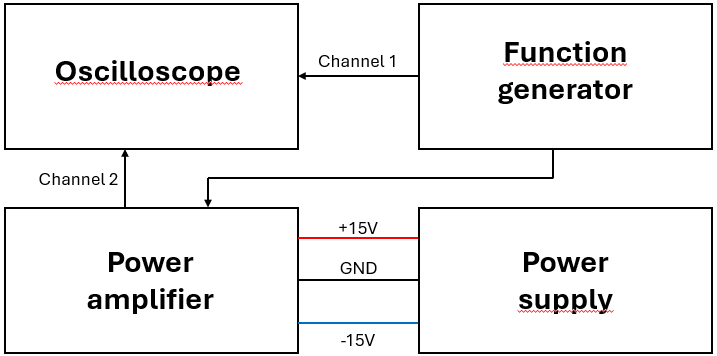
\includegraphics[width=0.8\linewidth]{TU Delft Booming Bass Project Report/figures/test setup.png}
    \caption{A schematic of the measuring setup used to analyze the performance of the power amplifier}
    \label{fig:PA test setup}
\end{figure}
%\begin{figure}[H]
%\centering
%\resizebox{0.75\textwidth}{!}{%
%\begin{circuitikz}
%\tikzstyle{every node}=[font=\Large]
%\draw  (2.75,18) rectangle (7,15.75);
%\draw  (10.5,18) rectangle (15,15.75);
%\draw  (2.75,14.25) rectangle (7,11.75);
%\draw  (10.5,14.25) rectangle (15,11.75);
%\draw [->, >=Stealth] (10.5,16.75) -- (7,16.75);
%\draw [->, >=Stealth] (5,14.25) -- (5,15.75);
%\draw [->, >=Stealth] (10.5,13) -- (7,13);
%\draw [->, >=Stealth] (10.5,13.75) -- (7,13.75);
%\draw [->, >=Stealth] (10.5,12.25) -- (7,12.25);
%\draw [short] (11.75,15.75) -- (11.75,15);
%\draw [short] (11.75,15) -- (6,15);
%\draw [->, >=Stealth] (6,15) -- (6,14.25);
%\end{circuitikz}
%}%
%\caption{a schematic of the measuring setup used to analyze the performance of the power amplifier}
%\label{fig:test setup}
%\end{figure}

The measurement procedure for the power amplifier circuit consisted of the following steps:
\begin{enumerate}
\item The input signal $\mathbf{V_{in}}$ from the Tektronix AFG 3021B/C function generator was connected at varying frequencies.
\item Both the input $\mathbf{V_{in}}$ and output $\mathbf{V_{out}}$ voltages were measured using the Tektronix TDS 2022B oscilloscope.
\item The gain was calculated by dividing the output voltage $\mathbf{V_{out}}$ by the input voltage $\mathbf{V_{in}}$.
\item The results from step 3 was then applied to \seautoref{eq: V to db}.

\end{enumerate}
 


\begin{figure}[h]
    \centering
    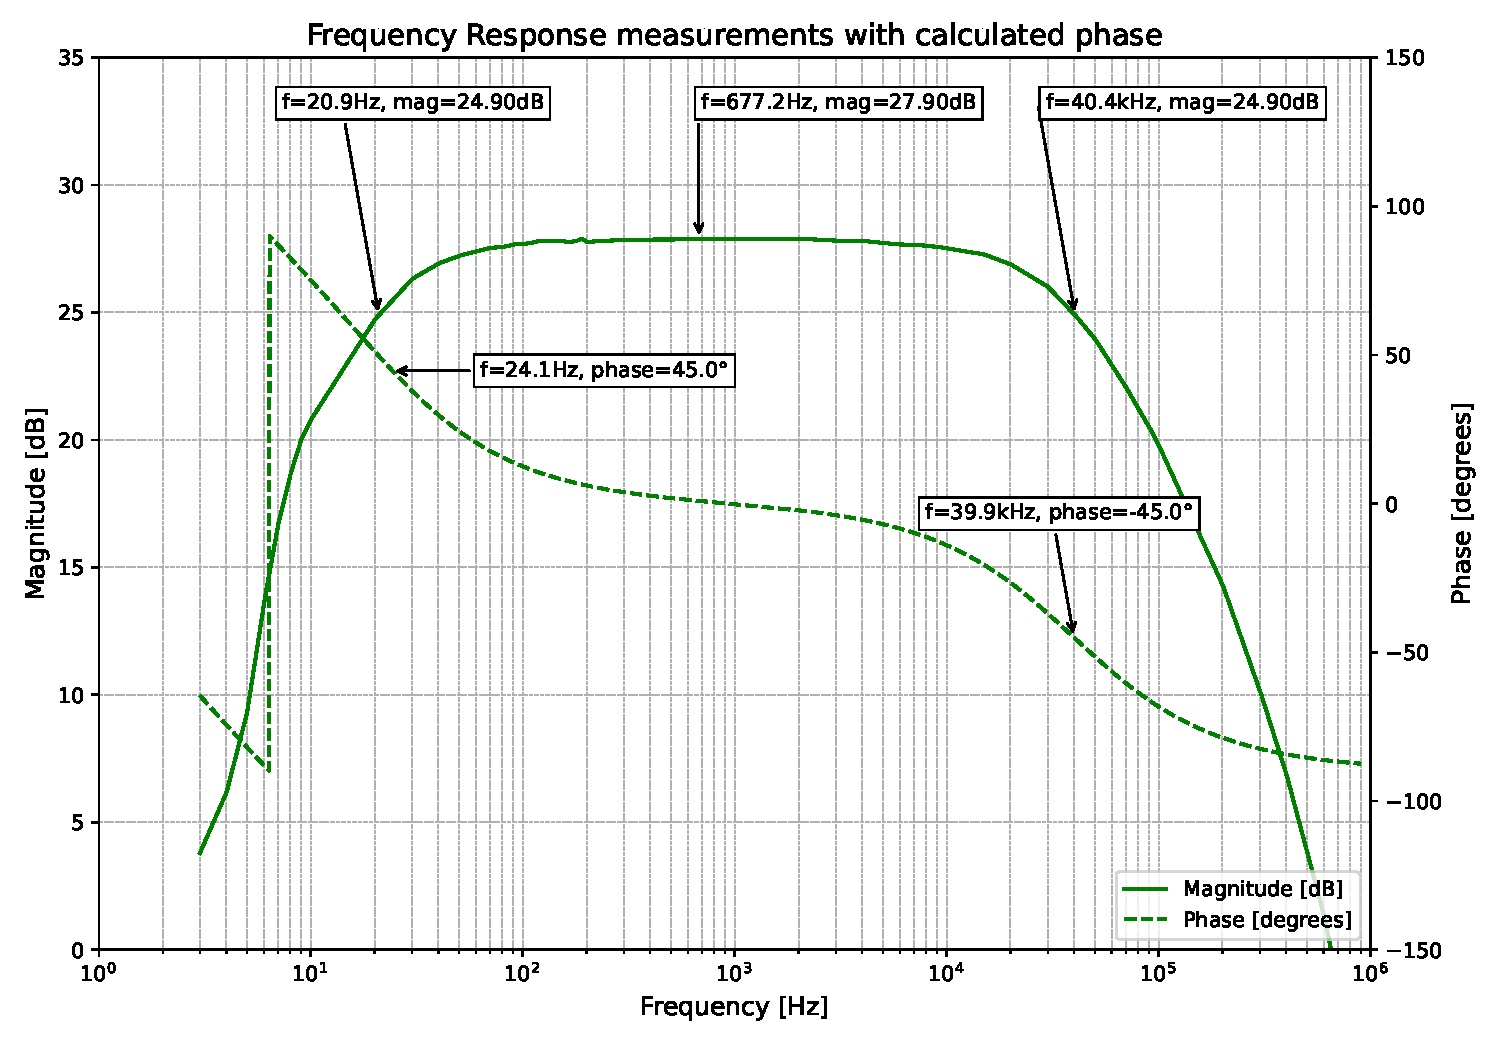
\includegraphics[width=0.9\linewidth]{TU Delft Booming Bass Project Report/figures/PowerAmplifier/measurements/metingen met misschien goede phase.pdf}
    \caption{Bode plot of measurements made with the power amplifier circuit of B2-1}
    \label{fig:freq response with phase}
\end{figure}

\subsubsection{B2-1 Final Results}

When examining, for example, \autoref{fig:40kHz}, the mean value of the sinusoidal voltage can be observed. In channel 1 (which represents the signal directly from the function generator), this mean value is approximately 500mV, while in channel 2 (the signal output from the power amplifier), the mean value is around 300mV. All of the measurements are summarized in \stautoref{tab:measurement_results}. To convert the measurement data into a continuous graph, MatplotLib was employed. The data points were transformed into a logarithmic scale to extrapolate 2000 entry points, which were then converted back into a linear scale. This process resulted in the graph shown in \sfautoref{fig:freq response with phase}.

\subsubsection{Obtaining the phase}
As demonstrated in \autoref{fig:20Hz} and \autoref{fig:40kHz}, a phase shift is observed between the output of the power amplifier and the function generator. Both signals are approximately in phase around 1kHz (see \sfautoref{fig:900Hz 400}). Plotting this phase shift based on the measurements proved to be difficult, so a function was created for use in Python to simplify the calculations (refer to \shortautoref{calculation of phase} for the code). This can be accomplished using \seautoref{eq: total transfer} (for the complete derivation of the phase equation, see \shortautoref{sec: phase calc}). The final phase plot is shown in \sfautoref{fig:freq response with phase}.

% In \sfautoref{fig:20Hz} and \sfautoref{fig:40kHz} two measurements can be seen, with a phase shift. Channel 1(the orange sinusoid) is from the function generator and channel 2 (the blue sinusoid) is the output of the power amplifier. An extra measurement where the phase is roughly the same between channel 1 and channel 2 can be seen in \sfautoref{fig:900Hz 400}


\begin{figure}[H]
\centering
\captionsetup{justification=raggedright, labelfont=bf}
\begin{subfigure}{.5\textwidth}
  \centering
    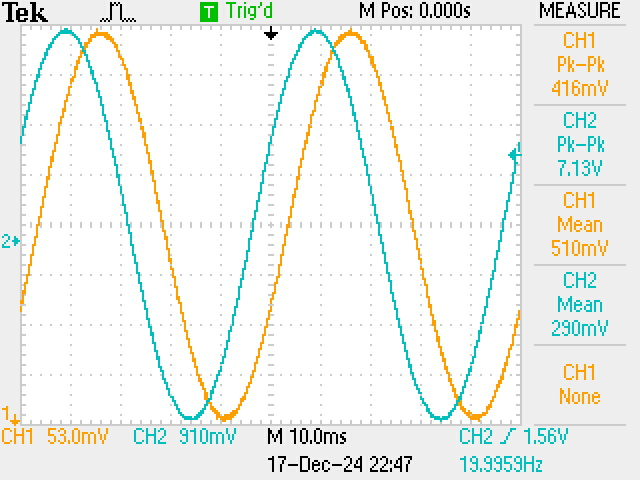
\includegraphics[width=0.95\linewidth]{TU Delft Booming Bass Project Report/figures/PowerAmplifier/measurements/20Hz.JPG}
    \captionsetup{justification=raggedright, labelfont=bf}
    \caption{A measurement with output from a function generator and the power amplifier at 20Hz.}
    \label{fig:20Hz}
\end{subfigure}%
\begin{subfigure}{.5\textwidth}
  \centering
    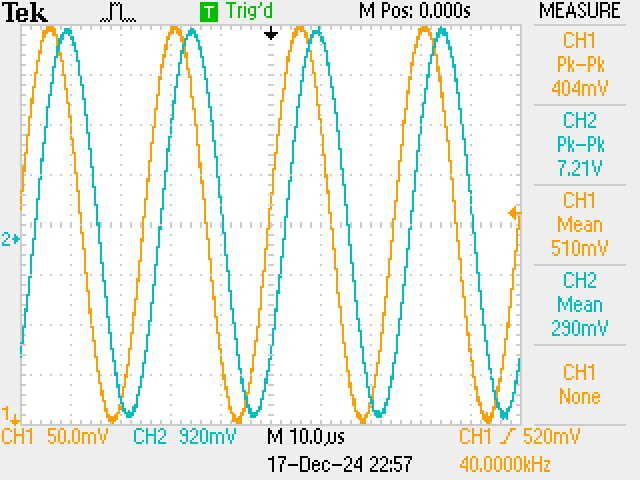
\includegraphics[width=0.95\linewidth]{TU Delft Booming Bass Project Report/figures/PowerAmplifier/measurements/40kHz.JPG}
    \captionsetup{justification=raggedright, labelfont=bf}
    \caption{A measurement with output from a function generator and the power amplifier at 40kHz.}
    \label{fig:40kHz}
\end{subfigure}
\caption{Two measurements showing the output of the function generator and B2-1's power amplifier at \~ 400mV, a clear phase shift is visible.}




\end{figure}

\begin{table}[H] % Ensures the table stays in place
\centering
\caption{Measurement Results from 3Hz to 900kHz of B2\_1's power amplifier}
\label{tab:measurement_results}
\begin{tabular}{|c|c||c|c||c|c|}
\hline
freq (Hz) & magnitude (dB) & freq (Hz) & magnitude (dB) & freq (Hz) & magnitude (dB) \\\hline
3 & 3.793281 & 150 & 27.809591 & 9000 & 27.576474 \\\hline
4 & 6.155268 & 160 & 27.767426 & 10000 & 27.515459 \\\hline
5 & 9.285681 & 170 & 27.767426 & 15000 & 27.276017 \\\hline
6 & 13.547177 & 180 & 27.809591 & 20000 & 26.890415 \\\hline
7 & 16.645216 & 190 & 27.895167 & 30000 & 26.010078 \\\hline
8 & 18.632909 & 200 & 27.767426 & 40000 & 24.936278 \\\hline
9 & 20.000000 & 300 & 27.853002 & 50000 & 23.974499 \\\hline
10 & 20.780155 & 400 & 27.853002 & 60000 & 22.937866 \\\hline
20 & 24.713002 & 500 & 27.853002 & 70000 & 22.079298 \\\hline
30 & 26.308784 & 600 & 27.895167 & 80000 & 21.255817 \\\hline
40 & 26.918908 & 700 & 27.895167 & 90000 & 20.525305 \\\hline
50 & 27.218201 & 800 & 27.895167 & 100000 & 19.803824 \\\hline
60 & 27.389528 & 900 & 27.895167 & 200000 & 14.341809 \\\hline
70 & 27.532069 & 1000 & 27.895167 & 300000 & 10.192336 \\\hline
80 & 27.557118 & 2000 & 27.895167 & 400000 & 6.915987 \\\hline
90 & 27.663610 & 3000 & 27.809591 & 500000 & 3.907928 \\\hline
100 & 27.681000 & 4000 & 27.809591 & 600000 & 1.413815 \\\hline
110 & 27.723164 & 5000 & 27.723164 & 700000 & -1.280346 \\\hline
120 & 27.809591 & 6000 & 27.662902 & 800000 & -3.262526 \\\hline
130 & 27.809591 & 7000 & 27.662902 & 900000 & -5.171004 \\\hline
140 & 27.809591 & 8000 & 27.618133 &  &  \\\hline
\end{tabular}
\end{table}

\subsubsection{B2-2 Final Design Results}

Some of the measurements of B2-2's power amplifier can be seen in \sfautoref{B2-2 PA measurements} and \sfautoref{fig:B2-2 3kHz}. The cut-off frequencies are at around 19.5Hz and 34kHz and the maximum voltage gain is about 26.6, or 28.5dB.
\begin{figure}[H]
\centering

\begin{subfigure}{.5\textwidth}
  \centering
    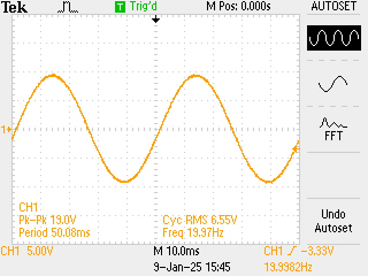
\includegraphics[width=0.95\linewidth]{TU Delft Booming Bass Project Report/figures/PowerAmplifier/measurements/Afbeelding1.png}
    \captionsetup{justification=raggedright, labelfont=bf}
    \caption{B2-2's measurement with output from the power amplifier at 20Hz.}
    \label{fig:B2-2 20Hz}
\end{subfigure}%
\begin{subfigure}{.5\textwidth}
  \centering
    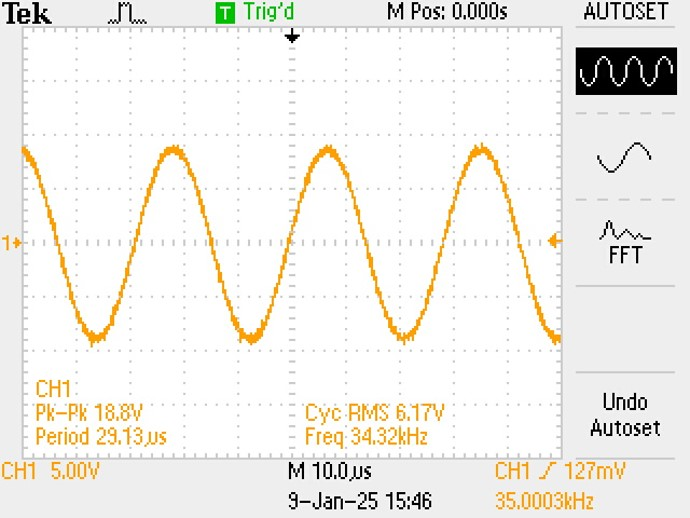
\includegraphics[width=0.95\linewidth]{TU Delft Booming Bass Project Report/figures/PowerAmplifier/measurements/Afbeelding2.jpg}
    \captionsetup{justification=raggedright, labelfont=bf}
    \caption{B2-2's measurement with output from the power amplifier at 35kHz.}
    \label{fig:B2-2 35kHz}
\end{subfigure}%
\captionsetup{justification=raggedright, labelfont=bf}
\caption{Two measurements showing the output of B2-2's power amplifier at 1V from the function generator.}
\label{B2-2 PA measurements}
\end{figure}

\subsubsection{Measurement at maximum gain}
\begin{figure}[H]
    \captionsetup{justification=raggedright, labelfont=bf}

\begin{subfigure}[t]{0.5\linewidth}
    \centering
    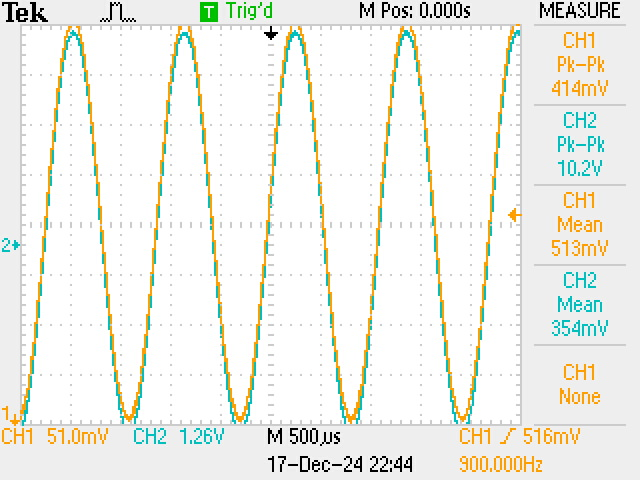
\includegraphics[width=0.9\linewidth]{TU Delft Booming Bass Project Report/figures/PowerAmplifier/measurements/900Hz.JPG}
    \caption{A measurement showing the output of the function generator and B2-1's power amplifier at \textasciitilde 400mV and 900Hz. Where the function generator and the power amplifier are almost in phase}
    \label{fig:900Hz 400}

\end{subfigure}
\begin{subfigure}[t]{0.5\linewidth}

  \centering
    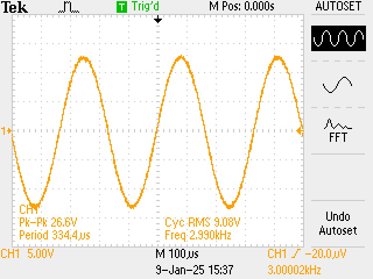
\includegraphics[width=0.9\linewidth]{TU Delft Booming Bass Project Report/figures/PowerAmplifier/measurements/Afbeelding3.png}
    \caption{B2-2's measurement with output from the power amplifier at 3kHz with 1V from the function generator.}
    \label{fig:B2-2 3kHz}

\captionsetup{justification=raggedright, labelfont=bf}
\label{B2 PA measurements 2}
\end{subfigure}
\caption{Two extra measurements of B2-1 and B2-2 power amplifier at around the maximum gain}

\end{figure}

\subsection{Filters}
The measurements serve as the key benchmark for evaluating the filter's quality. These measurements were collected throughout the filter design process, allowing for iterative adjustments. Ultimately, the final measurements included both acoustic and electric responses of the filters.

The acoustic measurements refer to the frequency-dependent response of the filter, which evaluates the power (in dB) of the acoustic signal emitted by the filter. On the other hand, the electric response involves analyzing the behavior of the filter across various frequencies, measured in terms of voltage gain (in dB).
\begin{figure}[H]
    \centering
    \begin{subfigure}[t]{0.48\textwidth}
        \centering
        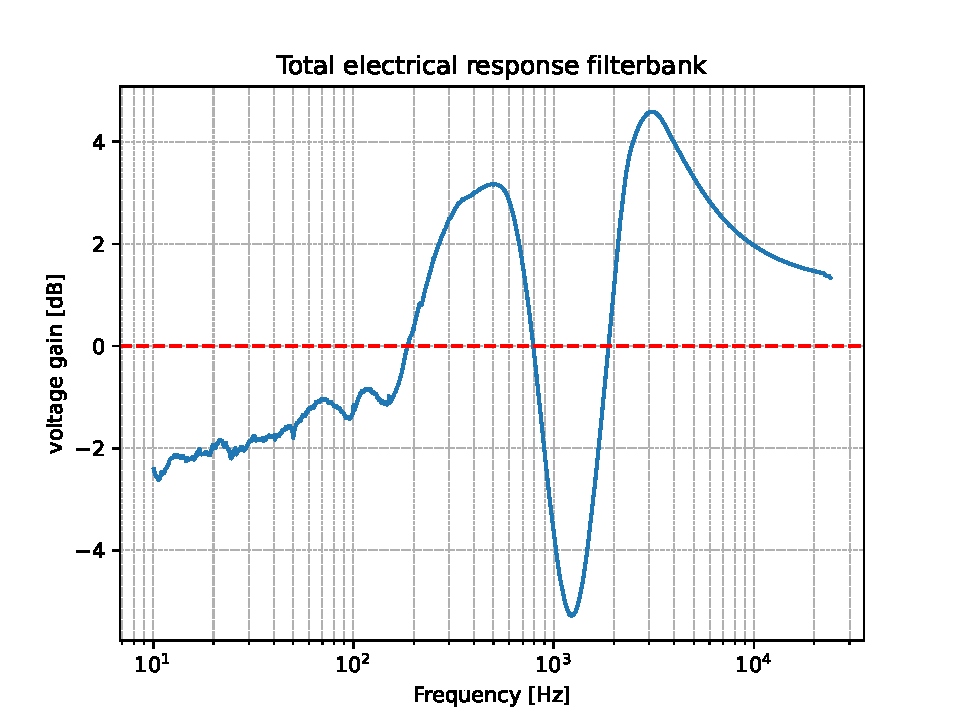
\includegraphics[width=\textwidth]{TU Delft Booming Bass Project Report/figures/FilterGroup/total_electric_response.pdf}
        \caption{The electric response of the filters.}
        \label{fig:electric_response}
    \end{subfigure}
    \hfill
    \begin{subfigure}[t]{0.48\textwidth}
        \centering
        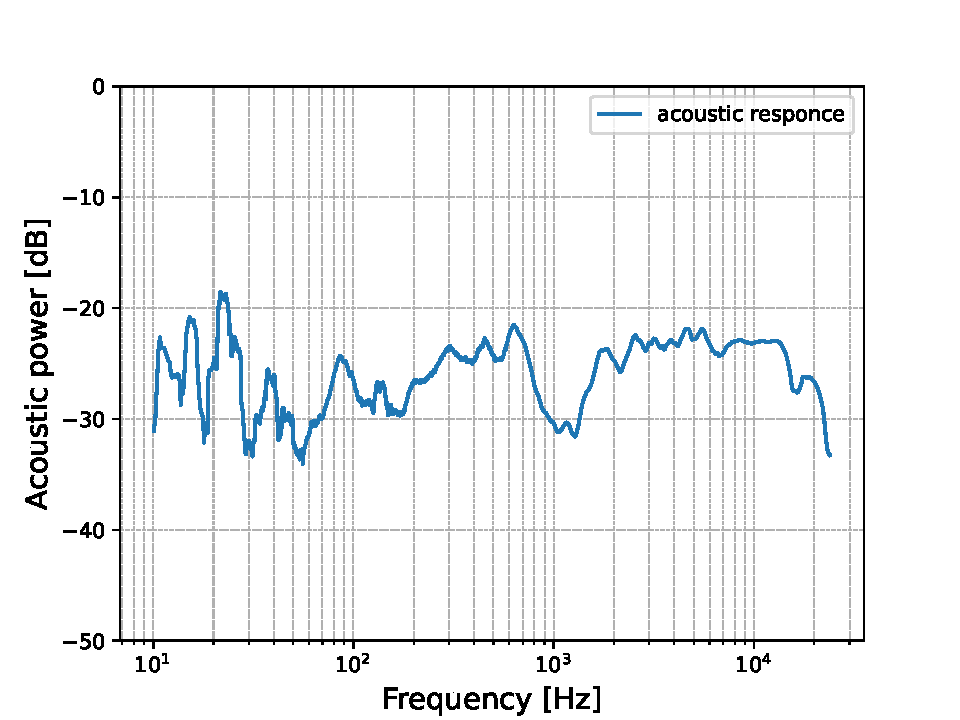
\includegraphics[width=\textwidth]{TU Delft Booming Bass Project Report/figures/FilterGroup/acoustic_response.pdf}
        \caption{The acoustic response of the filters shown at a 1-meter distance.}
        \label{fig:frequency_response}
    \end{subfigure}
    \captionsetup{justification=raggedright, labelfont=bf}
    \caption{A comparison of the electric and acoustic responses of the filters: (a) The electric response of the filters is depicted, showing the variations in the voltage gain across different frequencies. Significant changes in gain are observed, particularly at key frequency ranges, which could influence the overall performance of the system. (b) The acoustic response of the filters is shown at a 1-meter distance, illustrating how the system performs in terms of sound output and quality at this specific range.}
    \label{fig:combined_response}
\end{figure}

As observed in \sfautoref{fig:combined_response}, the electric response of the filters displays some inconsistencies. Notable gains occur around 500Hz and 1100Hz, while a dip in the voltage gain is evident between 800Hz and 1000Hz. This fluctuation may potentially impact the accuracy of the acoustic response, as it suggests a not-flat frequency response. Despite this, the acoustic response remains relatively flat, with fluctuations of approximately 10dB at max at around 1kHz. This deviation is directly attributed to the significant dip in the electric response seen in \sfautoref{fig:electric_response}. Furthermore, the decrease in acoustic power at this frequency range can be anticipated from the mid-band acoustic amplitude response in \sfautoref{fig: Cutoff frequencies}, where a similar reduction at 1000Hz aligns with both the electric and acoustic responses.

For the remained of the frequency range, the acoustic power remains relatively flat, with only minor dips and peaks. These slight variations are unlikely to significantly impact the overall sound quality of accuracy. Consequently, it can be concluded that the filters effectively contribute to the amplifier's ability to produce a more accurate and consistent sound profile.
